\documentclass{article}
\usepackage{caption}
\usepackage{cancel}
\usepackage{pifont}
\usepackage{tikz}
\usepackage[fontsize=16pt]{fontsize}

\author{Mike McLennan}
\date{}
\title{Simple\\Subtraction\\
\vspace{28pt}
\begin{normalsize}Applied Scholastics, Ferndale WA \end{normalsize}}

\begin{document}
\maketitle
\pagebreak
\tableofcontents
\pagebreak

\section{Subtraction}
Subtraction means taking away things. Subtract means to take away. The sub- means away, and the -tract means to pull, like with a tractor. To subtract a number is to take that value away from another number.\\

Minus means not having something or that something is less than something else, as in "Our team was minus our best player" or "the temperature is minus 3 degrees below zero." Minus is also another word for subtraction. The minus symbol $-$ is used in writing subtraction.\\

5 - 3 = 2 means that if have have 5 of something \ding{46}\ding{46}\ding{46}\ding{46}\ding{46} and take 3 of them away, \ding{46}\ding{46}\ding{46}or subtract them, then you are left with 2 of them. \ding{46}\ding{46} If you subtract 2 from 5 then you have 3 left.\\

Like the result of adding numbers is called the sum or the total, the result of subtracting one number from another is called the difference.

$$\underbrace{8}_{\textrm{number}} \overbrace{-}^{\textrm{minus}} \underbrace{3}_{\textrm{number}} = \overbrace{5}^{\textrm{difference}}$$
\vspace{28pt}

\pagebreak

If you subtract 3 from 8 and have 5 left, that is the same as saying that eight minus three leaves a difference of five. How different are 8 and 5? The difference is 3, and you write that as $8 - 3 = 5$.\\

Subtraction is the opposite of Addition. If you know your addition table for single-digit numbers then you already also know how to subtract them.\\

On a number line, subtraction can be shown by moving to the left:\\

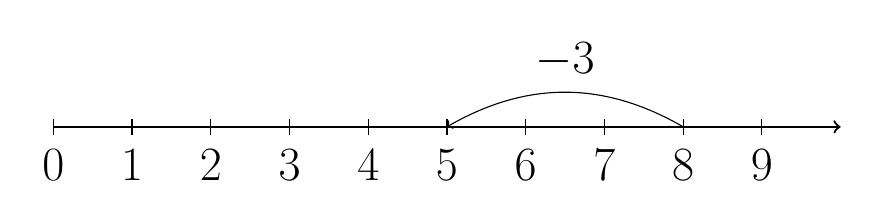
\begin{tikzpicture}
\draw[thick, ->] (0,0) -- (10,0) node[below] {$ $};
\foreach \n in {0,1,2,3,4,5,6,7,8,9} {\draw (\n,0.1) -- (\n,-0.1) node[below] {$\n$};}
\draw[->, bend right=30] (8,0) to node[above] {$-3$} (5,0);
\end{tikzpicture}

\begin{center}
$5 + 3 = 8$, so $8 - 3 = 5$
\end{center}

Of course, the first number has to be larger than the second number or the difference will be less than zero, which is another subject.

\pagebreak

\section{Subtraction in Columns}
Subtracting multi-digit numbers is done by arranging the numbers into columns that are all lined up with the ones-digits under each other. Then each column of digits is subtracted separately, starting with the ones, to get a difference.\\

$72 - 21$ can be solved by $7 - 2 = 5$ and $2 - 1 = 1$ resulting in a difference of 51:

\begin{center}
\begin{tabular}{c@{\,}c@{\,}c@{\,}}
 &7&2\\
-&2&1\\
\hline
=&5&1\\
\hline
\hline
\end{tabular}
\end{center}

\vspace{14pt}
The difference is separated by a single line, and is double underlined to indicate that this is a final answer.\\

Numbers, of any length, can be subtracted in this way. Keeping everything lined up  makes it a lot easier to do.

\begin{center}
\begin{tabular}{c@{\,}c@{\,}c@{\,}c@{\,}c@{\,}c@{\,}c@{\,}c@{\,}}
  & &1&0&4,&2&1&3\\
 -& & & &3,&1&1&2\\
\hline
= & &1&0&1,&1&0&1\\
\hline
\hline
\end{tabular}\\
\end{center}

\section{Borrowing}
In addition in columns sometimes a subtotal could be greater than 9 so that the tens digit had to be carried over to the next higher column.\\

We have the opposite problem in subtracting in columns. Sometimes the first number is smaller than the amount being taken away so the difference would be less than 0. It's solved by borrowing from the next highest column.

\begin{center}
\begin{tabular}{c@{\,}c@{\,}c@{\,}c@{\,}c}
& &1&^{4}\cancel{5}&^{1}3\\
   - & & &1&5\\
	\hline
	& & &3&7\\
	\hline
	\hline
\end{tabular}
\end{center}

\vspace{32pt}

Here is another example.\\

\begin{center}
\begin{tabular}{c@{\,}c@{\,}c@{\,}c@{\,}c}
&^2\cancel{3},&^{13}\cancel{4}&^{14}\cancel{5}&^{1}6\\
   - & &7&8&9\\
	\hline
	&2,&6&6&7\\
	\hline
	\hline
\end{tabular}
\end{center}

\pagebreak

As you can see, sometimes borrowing can get into chains of borrowing before the subtraction can be done.

\begin{center}
\begin{tabular}{c@{\,}c@{\,}c@{\,}c@{\,}c}
&^0\cancel{1},&^{9}\cancel{{^{1}0}}&^{9}\cancel{{{^1}0}}&^{1}0\\
   - & &7&8&9\\
	\hline
	&2,&6&6&7\\
	\hline
	\hline
\end{tabular}
\end{center}

\vspace{32pt}
Practice subtracting all sorts of numbers until you can do it easily and get it right every time!

\newpage
\

\begin{center}
\linespread{2}\large

Enquiries

\textbf{Applied Scholastics Ferndale}

Principal: Paula McLennan

mobile phone: 0431 683 306

email address: apsferndale@gmail.com

website: apsferndale.webs.com
\end{center}

\end{document}
